\chapter{Benchmark}
gfortran installieren:
\begin{lstlisting}[style=Bash]
$ sudo apt-get install gfortran sysfsutils cpufrequtils
\end{lstlisting}
cpu throttling deaktivieren. Wird von atlas verlangt:
\begin{lstlisting}[style=Bash]
$ sudo cpufreq-set -g performance
\end{lstlisting}
ATLAS installieren:
\begin{lstlisting}[style=Bash]
$ ./configure && make
\end{lstlisting}
hpcc downloaden:
\begin{lstlisting}[style=Bash]
$ wget http://icl.cs.utk.edu/projectsfiles/hpcc/download/hpcc-1.4.3.tar.gz
$ tar -xf hpcc-1.4.3.tar.gz
\end{lstlisting}
Make Konfiguration in hpl als Make.CoreI2 ablegen
\begin{lstlisting}[style=Bash]
...
\end{lstlisting}
Kompilieren:
\begin{lstlisting}[style=Bash]
$ make arch=CoreI2
\end{lstlisting}
Ausführen:
\begin{lstlisting}[style=Bash]
$ /shared/tools/openmpi/1.8.4/bin/mpirun -n 6 -hostfile /shared/mpi_hosts ./hpcc
\end{lstlisting}
Die theoretische Peak Performance liegt bei ca 1.8GHz*2(Cores)*3(Nodes)*4(FLOPs per cycle) = 43.2 Gflops.
Der unoptimierte Durchlauf erreicht 33.41 Gflops. Es werden 77\% der theoretischen Peak Performance erreicht.
Gründe hierfür sind unter anderen die langsame Kommunikation zwischen den CPUs und die langsame Speicheranbindung.\\
Ein mit icc kompilierter hpcc erreicht 33.41 Gflops.
\begin{lstlisting}[style=Bash]
$ /shared/tools/openmpi/1.8.4/bin/mpirun -n 6 -hostfile /shared/mpi_hosts ./hpcc
\end{lstlisting}
\section{iozone}
\begin{lstlisting}[style=Bash]
/etc/apt/sources.list non-free
# apt-get update
# apt-get install iozone3
iozone -a -i 0 -g 512M -F /shared/iotmp > out.txt
$ ./ GenGraph out.text
\end{lstlisting}
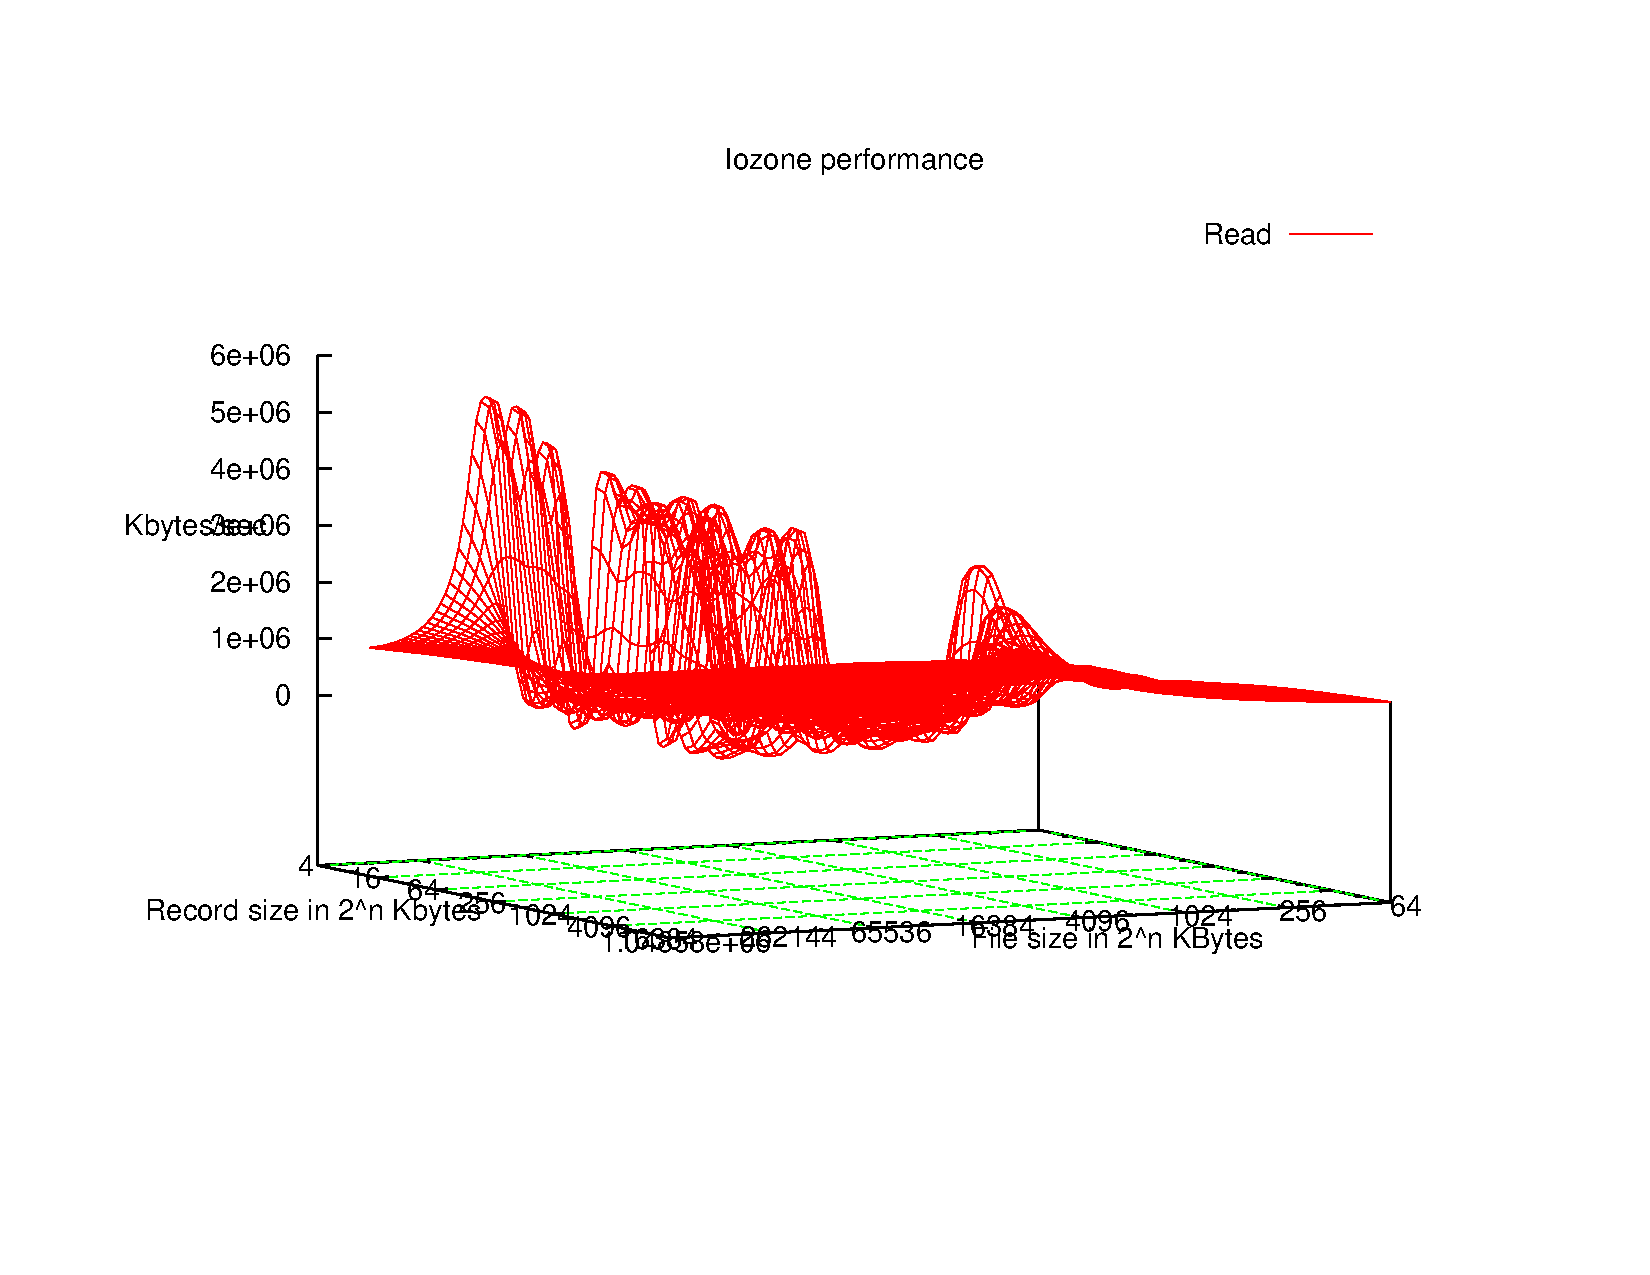
\includegraphics{read.pdf}
